\section{Introduction}

Unlike nodes in the Internet, cellular networks perform robust
authentication and network access control of all user devices on the
network. This control allows for cellular networks to provide tighter
guarantees on end-to-end quality of service and track each user's
consumption. These access logs are primarily maintained for the
purposes of billing, but also serve an important role to law
enforcement. Traditional telecommunications companies (telcos)
completely control this authentication and billing management within
their own centralized IT systems, known as the network core.

Community cellular networks are full stack cellular networks, using
the same protocols and user devices (cellphones) as national carriers,
but scoped for small rural communities where national carriers are not
incentivized to deploy their own
infrastructure.\cite{Heimerllongitudinalstudylocal2015} Due to their
rural nature, community cellular networks often cope with a slow and
intermittent backhaul connection between the edge community and the
network core. Assumptions of reliable connectivity between the cell
tower and the network core often break down in remote rural areas, and
standard approaches requiring updates to shared subscriber state in
the core do not allow the network to function when backhaul is down.
Such ``disconnected operation'' is highly desireable in rural
communities and disaster scenarios, where the ability to make a call
to a doctor in town or local emergency responders could be lifesaving.

Furthermore, community cellular networks face everyday challenges in
coordinating operation between a large number of small independent
communities. Local communities in the developing world have their own
local governance structures and network maintainers, but often want to
coordinate operation with other communities in the region to maximize
coverage, allow roaming, and make the sum of all networks more useful
for all the community members. This requires a protocol for
synchronizing network core state between the different communities,
and is complicated by the possibility that a user's particular home
community could go offline at any time (a contingency that traditional
telcos do not have to address).

My research is currently addressing both of these issues through the
development of an LTE packet core optimized for rural community
cellular networks. At the core of such a system is a distributed data
structure allowing both \emph{partioned operation} when a community is
offline and \emph{secure coordination} between independent communities.

\section{Approach}

My project combines the power of conflict free replicated data types
(CRDT)s for strong eventual consistency with a backing secure
distributed ledger for distributed coordination. Individual nodes
collect and batch signed state updates locally in a manner consistent
with CRDT principles, and then disseminate them to a backing secure
distributed ledger when they are online. This provides the following
capabilities distinctly applicable to rural community cellular networks

\begin{itemize}
\item Distributed global knowledge of transaction history to allow
  networks to manage the risk of serving any given user when offline.
\item Cryptographic assurance from the host network and each user that
  offline transactions are accurately recorded.
\item Consistent network core state at all times with bounded
  convergence to the accurate omniscient state.
\item Straightforward procedures for admitting new network operators
  and users to the network, with codable and enforceable policies to
  govern participant behavior on the network.
\item Replication of data and resilience to failures of individual
  community nodes.
\end{itemize}

\subsection{CRDT}
Conflict-Free Replicated Data Types are a class of data types which
have been shown to provide firm guarantees of Strong Eventual
Consistency.\cite{ShapiroConflictfreereplicateddata2011} A simple
example of a CRDT is a counter implementation, where instead of
storing the current value of the counter, the data structure tracks
individual increments and decrements. These same principles can be
applied to much more complicated data types, including nested and
structured data like JSON, while maintaining the same strong eventual
consistency guarantees.\cite{KleppmannConflictFreeReplicatedJSON2017}

New databases exist based on CRDTs designed to allow hyper-scale web
services spread across a wide geographic area to respond quickly to
queries where having the exact most up to date data is not essential
and the connection to other database replicas may be
unreliable.\cite{DatanetNewCRDT16} These databases provide a guarantee
that strong consistency can be achieved within a finite time window as
soon as connectivity is restored. As far as I have found, all current
implementations assume benign nodes and are optimized for performance
in a data center and web services context. While they tolerate
partitioned operation, they do not provide security guarantees towards
the accuracy and validity of the partitioned data in the presence of
malevolent actors.

\subsection{Secure Distributed Ledgers}
Colloquially referred to as ``blockchains,'' secure distributed
ledgers allow for nodes in a network to efficiently share a view of
global state in a completely distributed manner, without a trusted
intermediary, and in a way tolerant to failure and compromise of
individual nodes.\cite{BabuBlockchainTelco2016} Secure distributed
ledgers are most famous for their applications in crypto-currencies,
but the same techniques can be brought to bear in the context of
tracking any kind of centralized data shared between independent
actors. In the context of community networking, these ledgers
facilitate independent communities in a region banding together into a
large federated service provider with transparent roaming between the
communities.

\subsection{System Architecture}
My prototype implements a CRDT update based state store on top of a
distributed ledger. The system uses the hyperledger fabric framework
(https://github.com/hyperledger) to instantiate a private ledger. I
selected a private ledger architecture given that the local
communities have established (although loose) relationships and can
identify new community networks for admission to the ledger. In
contrast to true public ledgers on cryptocurrencies like Bitcoin or
Etherium, using a private ledger allows the system to avoid the
necessity of an expensive proof of work based consensus and ordering
mechanism. This is crucial for rural community networks in developing
regions where power often comes from generators or solar panels.

A hyperledger peer is deployed as a container to each community
network, handling synchronization of the local network state to the
global ledger when the network is online. All of the peers run an
agreed upon common ``chaincode'' which codifies the rules of
interacting with the network. My implemented chaincode validates each
CRDT update, checks that it is unique, and appends it to the
appropriate CRDT. Each hyperledger transaction is validated by
endorsing peers in the community, ensuring that peers check and agree
upon the validity of each transaction before it is committed.

As users interact with the local community network, they generate
usage entries detailing the amount of network resources
consumed. These entries are signed by both the user and the network,
and each hold a copy of the signed update in case the network is
offline. This ensures that at least one party is incentivized to
report all transactions that occur offline. Users are strongly
incentivized to report any additions or credit purchased, while the
network is strongly incentivized to report all usage to bill users for
their consumed network resources.

My prototype implements these signatures as a fake symmetric key
validation (simply checking that the registered key string is present)
to aid debugging for now, but is easily extensible to strong
cryptographic signatures.

\begin{figure*}[t]
  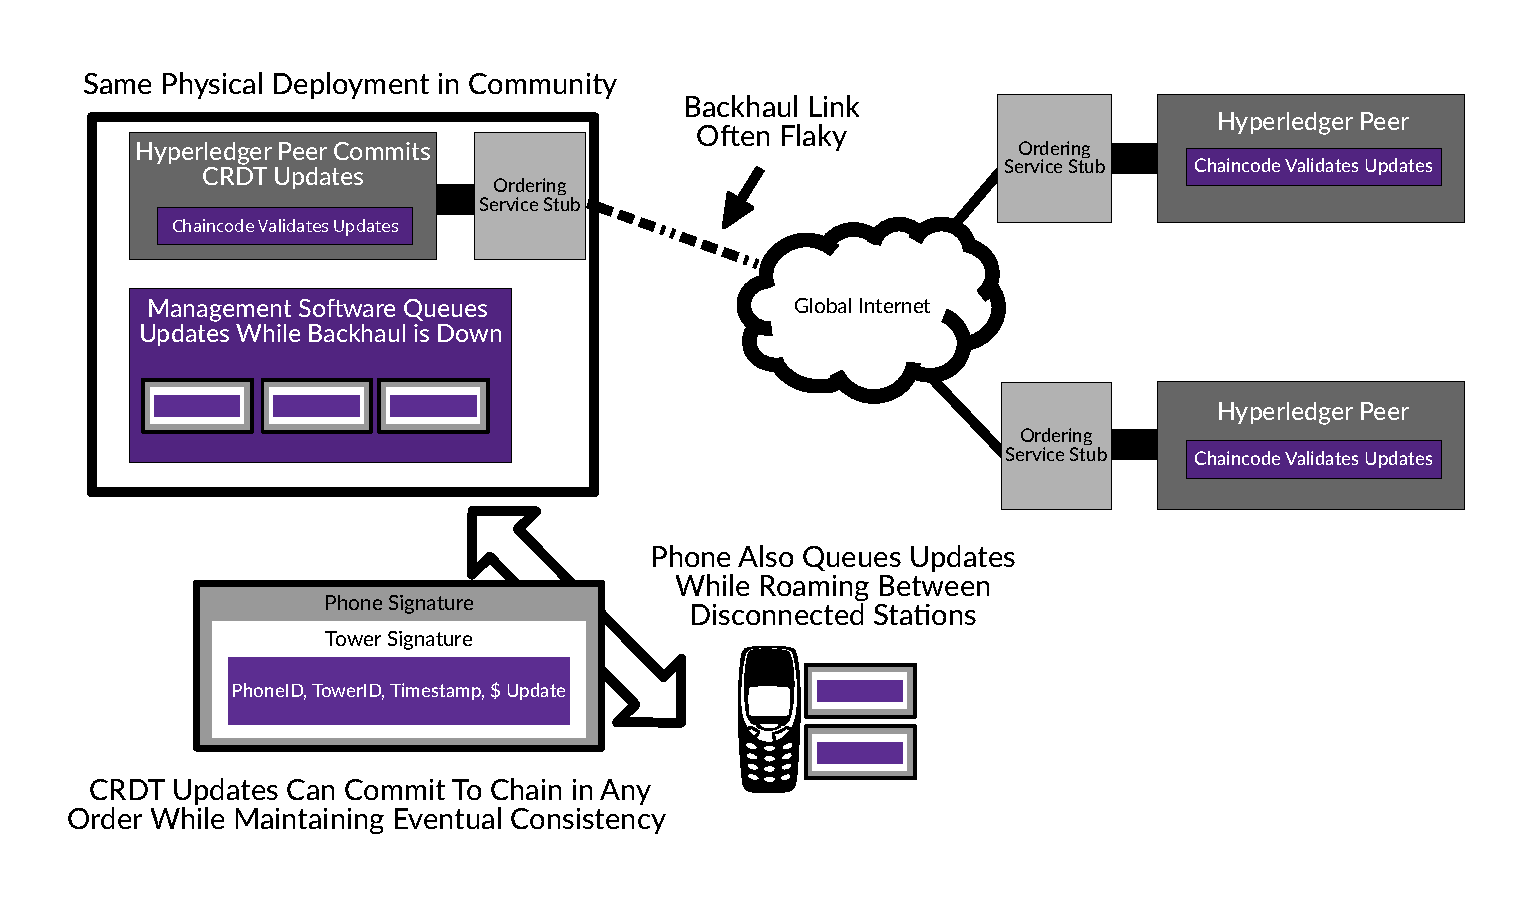
\includegraphics[width=\textwidth]{system-block-diagram}
  \caption{System block diagram}
\end{figure*}

\section{Related Work}
Many high level whitepapers cover the ``opportunities'' for
blockchains in
telecommunications\cite{BabuBlockchainTelco2016}\cite{BubleyBlockchainTelecomsIndustry2017}\cite{BaeOperatingmiddledigital},
but they seem to all be abstract consulting reports driven by
blockchain hype. There is one key academic paper by Jover and
Lackey\cite{JoverdHSSdistributedPeertoPeer2016a} which explores
building a Home Subscriber Server on a distributed ledger, but it does
not address intermittent backhaul and is only concerned with user
authentication, not user resource tracking as required to implement a
fully functioning network core. My work extends the concepts covered
by Jover and Lackey to provide the functionality required for a region
of rural telcos to coordinate seamless roaming and billing between
networks, even when individual networks are islanded from the rest of
the region. Leveraging existing concepts from theoretical
CRDTs\cite{ShapiroConflictfreereplicateddata2011}, this work presents
a novel CRDT based data storage architecture where individual updates
are signed and cached by users and the network before being
consolidated in a global ledger. This approach makes a different set
of tradeoffs to achieve distinct end goals from existing CRDT database
implementations.\cite{DatanetNewCRDT16} My prototype system incurrs
additional overhead by maintaining global state in a secure ledger as
compared to a traditional database, but this model better maps to the
independent governance models of rural community networks.

\section{Current Progress}

So far I have successfully setup a hyperledger fabric development
environment, developed the necessary chaincode to validate, commint,
and query the CRDT updates, and tested the chaincode in a hyperledger
network running in containers on my personal computer. I have begun
development of the local queuing component, but have not tested it end
to end with the backing ledger. I believe I am on track to be able to
test the performance of my prototype system in time for the poster
session in two weeks.

\subsection{Challenges}

The biggest challenges for me so far have been related to learning how
to develop in the hyperledger environment and learn how the fabric
framework exposes different ledger concepts. Hyperledger fabric is
relatively new, so while there are some tutorials available, they are
not very mature and documentation is actively under development.

\section{Remaining Quarter Plan}

I plan to spend 1-2 more days developing the middle management layer
to handle queuing of updates while the local network is offline, and
do not anticipate much trouble with it now that I have a working and
repeatable fabric environment. After that I will finish HW4, and then
plan to spend the last week and a half conducting the evaluation below
and preparing my poster.

\subsection{Evaluation Plan}

I plan to evaluate my system across two classes of requirements:
``absolute requirements'' and ``performance requirements''. Absolute
requirements are either met or not met by the system. I will evaluate
these requirements through the construction of test cases for each one
and report on if my constructed prototype meets each requirement in
the final presentation. If my prototype does not meet any of the
absolute requirements, I will explain why it does not, and propose a
potential solution to explore in future work.

Currently the only absolute requirements are:
\begin{itemize}
\item The system must be deployable on a community network basestation
  with 8GB ram, a single quad core processor, and a solid state disk.
\item The system must support offline operation.
\item The system must maintain strong eventual consistency at all
  times under byzantine failure.
\end{itemize}

Performance requirements are related to the performance of my system
implementation and the way the system scales with additional
demand. Performance requirements depend on the amount and
characteristics of traffic, and will be evaluated through measurements
at multiple traffic magnitudes to determine the trend in performance
as traffic/demand increases where relevant.

Performance metrics in the distributed system will also change as the
number of peer nodes in the system varies, which I will measure by
repeating measurements with a variable number of peer nodes
operational in the network. The docker based implementation of the
network easily allows me to increase the number of participating
nodes on a single development machine.

I plan to measure the following performance metrics with simulated
traffic on a dual core (hyperthreaded) development machine with 16GB
of ram and a solid state disk:
\begin{itemize}
\item CPU utilization trend peak/avg
\item RAM utilization trend peak/avg
\item Disk io throughput trend peak/avg
\item Disk utilization per transaction
\item Network traffic per transaction
\item Maximum steady state number of updates processed per second
\end{itemize}

I will gather the measurements with available unix resource
utilization utilities (htop, iotop, nettop), through traces of the
active network traffic during a transaction (wireshark), and through
instrumentation of the filesystem to observe file size changes as
updates are processed.

%%% Local Variables:
%%% mode: latex
%%% TeX-master: "main"
%%% End:
